% questions.tex —— 2020 年·全国Ⅰ卷·理科 · 题目内容片段（无答案）
% 由 tools/generate_projects.py 依来源总账自 2020/2020_数学真题_理_试题.md 生成，勿手改（改源 MD 后重跑）


\begin{gknotice}
\textbf{ 卷种提示（务必先读）}

本卷为\textbf{文理分科时代的旧结构}：12 道单选（无多选）+ 4 填空 + 5 道必做解答题 + \textbf{第 22/23 题二选一的「选做题」}。

\textbf{选做题（极坐标与参数方程 / 不等式选讲）在现行新课标中已取消}，2021 年起的新高考 I 卷不再考查。本卷第 22、23 题仅作历史资料保留，\textbf{不建议练习}。

其余题目的知识点仍在考纲内，适合\textbf{按知识点抽题}使用，不适合整套限时模拟。

\textbf{适用省份}：河南、河北、山西、江西、湖北、湖南、广东、安徽、福建
\end{gknotice}

\par\medskip

\gkpart{一、选择题}

\begin{gktip}
本题共 12 小题，每小题 5 分，共 60 分。在每小题给出的四个选项中，只有一项是符合题目要求的。
\end{gktip}

\begin{question}
\gkti{1}若 $z=1+\mathrm i$，则 $\left|z^{2}-2z\right|=$（　　）

\begin{gkopts}(4)
\task A．$0$
\task B．$1$
\task C．$\sqrt2$
\task D．$2$
\end{gkopts}

\end{question}
\begin{question}
\gkti{2}设集合 $A=\left\{x\mid x^{2}-4\le0\right\}$，$B=\{x\mid2x+a\le0\}$，且 $A\cap B=\{x\mid-2\le x\le1\}$，则 $a=$（　　）

\begin{gkopts}(4)
\task A．$-4$
\task B．$-2$
\task C．$2$
\task D．$4$
\end{gkopts}

\end{question}
\begin{question}
\gkti{3}埃及胡夫金字塔是古代世界建筑奇迹之一，它的形状可视为一个正四棱锥，以该四棱锥的高为边长的正方形面积等于该四棱锥一个侧面三角形的面积，则其侧面三角形底边上的高与底面正方形的边长的比值为（　　）

\begin{gkopts}(2)
\task A．$\dfrac{\sqrt5-1}4$
\task B．$\dfrac{\sqrt5-1}2$
\task C．$\dfrac{\sqrt5+1}4$
\task D．$\dfrac{\sqrt5+1}2$
\end{gkopts}

\end{question}
\begin{question}
\gkti{4}已知 $A$ 为抛物线 $C:y^{2}=2px\ (p>0)$ 上一点，点 $A$ 到 $C$ 的焦点的距离为 $12$，到 $y$ 轴的距离为 $9$，则 $p=$（　　）

\begin{gkopts}(4)
\task A．$2$
\task B．$3$
\task C．$6$
\task D．$9$
\end{gkopts}

\Needspace{0.4\textheight}
\end{question}
\begin{question}
\gkti{5}某校一个课外学习小组为研究某作物种子的发芽率 $y$ 和温度 $x$（单位：$^\circ\mathrm C$）的关系，在 $20$ 个不同的温度条件下进行种子发芽实验，由实验数据 $\left(x_i,y_i\right)\ (i=1,2,\cdots,20)$ 得到下面的散点图：
\nopagebreak[4]
\begin{center}% 2020 全国Ⅰ卷 理5：发芽率-温度散点图（对数饱和形态，数据点按原图形态示意布点）
\begin{tikzpicture}
\begin{axis}[width=8.8cm, height=5cm, font=\small,
  xlabel={温度$/^{\circ}\mathrm{C}$}, ylabel={发芽率},
  xlabel style={at={(1,0)}, anchor=north west},
  ylabel style={at={(0,1)}, anchor=south, rotate=-90},
  xmin=0, xmax=44, ymin=0, ymax=1.08,
  xtick={0,10,20,30,40},
  ytick={0.2,0.4,0.6,0.8,1.0},
  yticklabels={$20\%$,$40\%$,$60\%$,$80\%$,$100\%$},
  axis lines=left, axis line style={-Stealth}]
  \addplot[only marks, mark=square*, mark size=1.3pt] coordinates {
    (10,0.36) (11.5,0.42) (13,0.50) (14.5,0.55) (16,0.58)
    (17.5,0.62) (19,0.64) (20.5,0.68) (22,0.69) (23.5,0.72)
    (25,0.73) (26.5,0.76) (28,0.76) (29.5,0.79) (31,0.80)
    (33,0.82) (35,0.83) (37,0.86) (39,0.86) (40.5,0.88)};
  \addplot[domain=9:41, samples=80, smooth] {0.35*ln(x)-0.45};
\end{axis}
\end{tikzpicture}
\end{center}
\nopagebreak[4]
由此散点图，在 $10\ ^\circ\mathrm C$ 至 $40\ ^\circ\mathrm C$ 之间，下面四个回归方程类型中最适宜作为发芽率 $y$ 和温度 $x$ 的回归方程类型的是（　　）

\begin{gkopts}(2)
\task A．$y=a+bx$
\task B．$y=a+bx^{2}$
\task C．$y=a+b\mathrm e^{x}$
\task D．$y=a+b\ln x$
\end{gkopts}

\end{question}
\begin{question}
\gkti{6}函数 $f(x)=x^{4}-2x^{3}$ 的图象在点 $(1,f(1))$ 处的切线方程为（　　）

\begin{gkopts}(4)
\task A．$y=-2x-1$
\task B．$y=-2x+1$
\task C．$y=2x-3$
\task D．$y=2x+1$
\end{gkopts}

\Needspace{0.4\textheight}
\end{question}
\begin{question}
\gkti{7}设函数 $f(x)=\cos\left(\omega x+\dfrac\pi6\right)$ 在 $[-\pi,\pi]$ 的图象大致如下图，则 $f(x)$ 的最小正周期为（　　）
\nopagebreak[4]
\begin{center}% 2020 全国Ⅰ卷 理7：f(x)=cos(ωx+π/6) 的图象（按答案 T=4π/3，即 ω=3/2 精确绘制）
\begin{tikzpicture}
\begin{axis}[width=8.6cm, height=4.6cm, font=\small,
  axis lines=middle, xlabel={$x$}, ylabel={$y$},
  xmin=-3.6, xmax=3.7, ymin=-1.35, ymax=1.45,
  xtick={-3.14159, -1.39626, 3.14159},
  xticklabels={$-\pi$, $-\frac{4\pi}{9}$, $\pi$},
  ytick=\empty,
  every axis x label/.style={at={(current axis.right of origin)}, anchor=west},
  every axis y label/.style={at={(current axis.above origin)}, anchor=south}]
  \addplot[domain=-3.14159:3.14159, samples=200, thick] {cos(deg(1.5*x + pi/6))};
  \node[below left, font=\small] at (axis cs:0,0) {$O$};
\end{axis}
\end{tikzpicture}
\end{center}
\nopagebreak[4]
\begin{gkopts}(4)
\task A．$\dfrac{10\pi}9$
\task B．$\dfrac{7\pi}6$
\task C．$\dfrac{4\pi}3$
\task D．$\dfrac{3\pi}2$
\end{gkopts}

\end{question}
\begin{question}
\gkti{8}$\left(x+\dfrac{y^{2}}x\right)(x+y)^{5}$ 的展开式中 $x^{3}y^{3}$ 的系数为（　　）

\begin{gkopts}(4)
\task A．$5$
\task B．$10$
\task C．$15$
\task D．$20$
\end{gkopts}

\end{question}
\begin{question}
\gkti{9}已知 $\alpha\in(0,\pi)$，且 $3\cos2\alpha-8\cos\alpha=5$，则 $\sin\alpha=$（　　）

\begin{gkopts}(2)
\task A．$\dfrac{\sqrt5}3$
\task B．$\dfrac23$
\task C．$\dfrac13$
\task D．$\dfrac{\sqrt5}9$
\end{gkopts}

\end{question}
\begin{question}
\gkti{10}已知 $A$，$B$，$C$ 为球 $O$ 的球面上的三个点，$\odot O_1$ 为 $\triangle ABC$ 的外接圆。若 $\odot O_1$ 的面积为 $4\pi$，$AB=BC=AC=OO_1$，则球 $O$ 的表面积为（　　）

\begin{gkopts}(4)
\task A．$64\pi$
\task B．$48\pi$
\task C．$36\pi$
\task D．$32\pi$
\end{gkopts}

\end{question}
\begin{question}
\gkti{11}已知 $\odot M:x^{2}+y^{2}-2x-2y-2=0$，直线 $l:2x+y+2=0$，$P$ 为 $l$ 上的动点。过点 $P$ 作 $\odot M$ 的切线 $PA$，$PB$，切点为 $A$，$B$，当 $|PM|\cdot|AB|$ 最小时，直线 $AB$ 的方程为（　　）

\begin{gkopts}(4)
\task A．$2x-y-1=0$
\task B．$2x+y-1=0$
\task C．$2x-y+1=0$
\task D．$2x+y+1=0$
\end{gkopts}

\end{question}
\begin{question}
\gkti{12}若 $2^{a}+\log_2 a=4^{b}+2\log_4 b$，则（　　）

\begin{gkopts}(4)
\task A．$a>2b$
\task B．$a<2b$
\task C．$a>b^{2}$
\task D．$a<b^{2}$
\end{gkopts}

\par\medskip

\end{question}
\gkpart{二、填空题}

\begin{gktip}
本题共 4 小题，每小题 5 分，共 20 分。
\end{gktip}

\begin{question}
\gkti{13}若 $x$，$y$ 满足约束条件 $\begin{cases}2x+y-2\le0\\ x-y-1\ge0\\ y+1\ge0\end{cases}$，则 $z=x+7y$ 的最大值为 \gkblank{}．

\end{question}
\begin{question}
\gkti{14}设 $\boldsymbol a$，$\boldsymbol b$ 为单位向量，且 $|\boldsymbol a+\boldsymbol b|=1$，则 $|\boldsymbol a-\boldsymbol b|=$ \gkblank{}．

\end{question}
\begin{question}
\gkti{15}已知 $F$ 为双曲线 $C:\dfrac{x^{2}}{a^{2}}-\dfrac{y^{2}}{b^{2}}=1\ (a>0,\ b>0)$ 的右焦点，$A$ 为 $C$ 的右顶点，$B$ 为 $C$ 上的点，且 $BF$ 垂直于 $x$ 轴。若 $AB$ 的斜率为 $3$，则 $C$ 的离心率为 \gkblank{}．

\Needspace{0.4\textheight}
\end{question}
\begin{question}
\gkti{16}如图，在三棱锥 $P\text{-}ABC$ 的平面展开图中，$AC=1$，$AB=AD=\sqrt3$，$AB\perp AC$，$AB\perp AD$，$\angle CAE=30^\circ$，则 $\cos\angle FCB=$ \gkblank{}．
\nopagebreak[4]
\begin{center}% 2020 全国Ⅰ卷 理16：三棱锥 P-ABC 的平面展开图
% 依题给条件重建：AC=1、AB=AD=√3、AB⊥AC、AB⊥AD、∠CAE=30°、AE=√3；
% D、E、F 折起后重合于顶点 P（原库位图裁切损坏，本图按几何条件精确重绘）
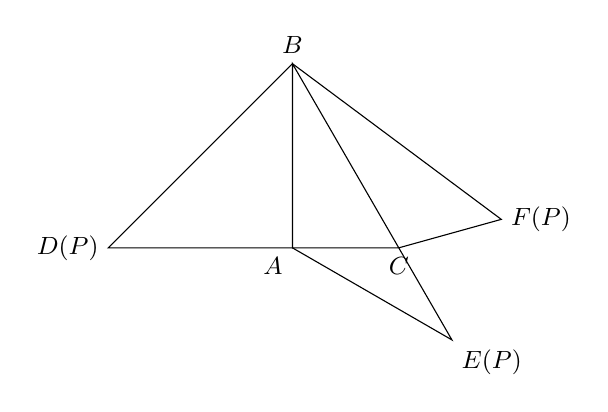
\begin{tikzpicture}[scale=1.35, font=\small]
  \coordinate (A) at (0,0);
  \coordinate (B) at (0,1.7320508);
  \coordinate (C) at (1,0);
  \coordinate (D) at (-1.7320508,0);
  \coordinate (E) at (1.5,-0.8660254);   % √3·(cos(-30°),sin(-30°))
  \coordinate (F) at (1.9641,0.2679);    % 由 FC=EC=1、FB=DB=√6 解出
  \draw (A) -- (B) -- (C) -- cycle;      % 中心三角形（折痕）
  \draw (B) -- (D) -- (A);               % △DAB
  \draw (A) -- (E) -- (C);               % △AEC
  \draw (C) -- (F) -- (B);               % △CFB
  \node[below left]  at (A) {$A$};
  \node[above]       at (B) {$B$};
  \node[below]       at (C) {$C$};
  \node[left]        at (D) {$D(P)$};
  \node[below right] at (E) {$E(P)$};
  \node[right]       at (F) {$F(P)$};
\end{tikzpicture}
\end{center}
\nopagebreak[4]
\par\medskip

\end{question}
\gkpart{三、解答题}

\begin{gktip}
共 70 分。解答应写出文字说明、证明过程或演算步骤。第 17～21 题为必考题，每个试题考生都必须作答。第 22、23 题为选考题，考生根据要求作答。
\end{gktip}

\gksubpart{（一）必考题：共 60 分}

\begin{question}
\gkti{17}\textbf{（12 分）} 设 $\left\{a_n\right\}$ 是公比不为 $1$ 的等比数列，$a_1$ 为 $a_2$，$a_3$ 的等差中项。

  (1) 求 $\left\{a_n\right\}$ 的公比；

  (2) 若 $a_1=1$，求数列 $\left\{na_n\right\}$ 的前 $n$ 项和。

\Needspace{0.4\textheight}
\end{question}
\begin{question}
\gkti{18}\textbf{（12 分）} 如图，$D$ 为圆锥的顶点，$O$ 是圆锥底面的圆心，$AE$ 为底面直径，$AE=AD$。$\triangle ABC$ 是底面的内接正三角形，$P$ 为 $DO$ 上一点，$PO=\dfrac{\sqrt6}6DO$。
\nopagebreak[4]
\begin{center}% 2020 全国Ⅰ卷 理18：圆锥（顶点 D，底面圆心 O，AE 为直径，△ABC 内接正三角形，P 在 DO 上）
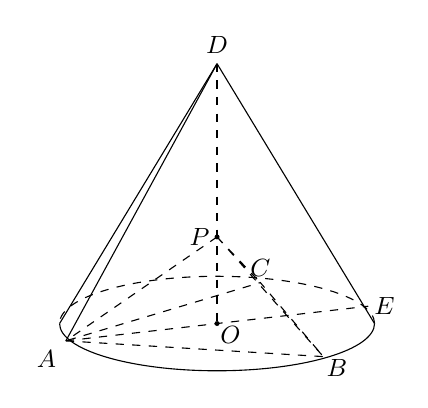
\begin{tikzpicture}[scale=1.0, font=\small]
  \coordinate (D) at (0,3.3);
  \coordinate (O) at (0,0);
  \coordinate (A) at (-1.92,-0.22);
  \coordinate (E) at (1.92,0.22);
  \coordinate (B) at (1.35,-0.42);
  \coordinate (C) at (0.55,0.52);
  \coordinate (P) at (0,1.1);
  % 底面椭圆：前半实、后半虚
  \draw (-2,0) arc (180:360:2 and 0.6);
  \draw[dashed] (2,0) arc (0:180:2 and 0.6);
  % 锥面轮廓
  \draw (D) -- (-2,0);
  \draw (D) -- (2,0);
  % 中轴与内部连线
  \draw[dashed] (D) -- (O);
  \draw[dashed] (A) -- (E);
  \draw[dashed] (A) -- (B) -- (C) -- cycle;
  \draw[dashed] (P) -- (A)  (P) -- (B)  (P) -- (C);
  \draw (D) -- (A);
  \fill (O) circle (0.9pt);  \fill (P) circle (0.9pt);
  \node[above] at (D) {$D$};
  \node[below left] at (A) {$A$};
  \node[below right, inner sep=1pt] at (B) {$B$};
  \node[right, inner sep=2pt] at (E) {$E$};
  \node[above, inner sep=2pt] at (C) {$C$};
  \node[below right, inner sep=1pt] at (O) {$O$};
  \node[left, inner sep=2.5pt] at (P) {$P$};
\end{tikzpicture}
\end{center}
\nopagebreak[4]
  (1) 证明：$PA\perp$ 平面 $PBC$；

  (2) 求二面角 $B\text{-}PC\text{-}E$ 的余弦值。

\end{question}
\begin{question}
\gkti{19}\textbf{（12 分）} 甲、乙、丙三位同学进行羽毛球比赛，约定赛制如下：累计负两场者被淘汰；比赛前抽签决定首先比赛的两人，另一人轮空；每场比赛的胜者与轮空者进行下一场比赛，负者下一场轮空，直至有一人被淘汰；当一人被淘汰后，剩余的两人继续比赛，直至其中一人被淘汰，另一人最终获胜，比赛结束。经抽签，甲、乙首先比赛，丙轮空。设每场比赛双方获胜的概率都为 $\dfrac12$。

  (1) 求甲连胜四场的概率；

  (2) 求需要进行第五场比赛的概率；

  (3) 求丙最终获胜的概率。

\end{question}
\begin{question}
\gkti{20}\textbf{（12 分）} 已知 $A$，$B$ 分别为椭圆 $E:\dfrac{x^{2}}{a^{2}}+y^{2}=1\ (a>1)$ 的左、右顶点，$G$ 为 $E$ 的上顶点，$\overrightarrow{AG}\cdot\overrightarrow{GB}=8$，$P$ 为直线 $x=6$ 上的动点，$PA$ 与 $E$ 的另一交点为 $C$，$PB$ 与 $E$ 的另一交点为 $D$。

  (1) 求 $E$ 的方程；

  (2) 证明：直线 $CD$ 过定点。

\end{question}
\begin{question}
\gkti{21}\textbf{（12 分）} 已知函数 $f(x)=\mathrm e^{x}+ax^{2}-x$。

  (1) 当 $a=1$ 时，讨论 $f(x)$ 的单调性；

  (2) 当 $x\ge0$ 时，$f(x)\ge\dfrac12x^{3}+1$，求 $a$ 的取值范围。

\par\medskip

\end{question}
\gksubpart{（二）选考题：共 10 分，请考生在第 22、23 题中任选一题作答}

\begin{gktip}
\textbf{ 现行考纲已取消选做题}，以下两题仅作历史资料保留，不建议练习。
\end{gktip}

\begin{question}
\gkti{22}\textbf{（10 分）〔选修 4-4：坐标系与参数方程〕} （\textbf{已取消}）

在直角坐标系 $xOy$ 中，曲线 $C_1$ 的参数方程为 $\begin{cases}x=\cos^{k}t\\ y=\sin^{k}t\end{cases}$（$t$ 为参数）。以坐标原点为极点，$x$ 轴正半轴为极轴建立极坐标系，曲线 $C_2$ 的极坐标方程为 $4\rho\cos\theta-16\rho\sin\theta+3=0$。

  (1) 当 $k=1$ 时，$C_1$ 是什么曲线？

  (2) 当 $k=4$ 时，求 $C_1$ 与 $C_2$ 的公共点的直角坐标。

\end{question}
\begin{question}
\gkti{23}\textbf{（10 分）〔选修 4-5：不等式选讲〕} （\textbf{已取消}）

已知函数 $f(x)=|3x+1|-2|x-1|$。

  (1) 画出 $y=f(x)$ 的图象；

  (2) 求不等式 $f(x)>f(x+1)$ 的解集。

\par\medskip


\end{question}